%% This Beamer template is based on the one found here: https://github.com/sanhacheong/stanford-beamer-presentation, and edited to be used for Stanford ARM Lab

\documentclass[10pt, aspectratio=169]{beamer}
%\mode<presentation>{}

\usepackage{media9}
\usepackage{amssymb,amsmath,amsthm,enumerate}
\usepackage[utf8]{inputenc}
\usepackage{array}
\usepackage[parfill]{parskip}
\usepackage{graphicx}
\usepackage{caption}
\usepackage{subcaption}
\usepackage{bm}
\usepackage{amsfonts,amscd}
\usepackage[]{units}
\usepackage{listings}
\usepackage{multicol}
\usepackage{multirow}
\usepackage{tcolorbox}
\usepackage{physics}

% Enable colored hyperlinks
\hypersetup{
    colorlinks=true,
    citecolor=uma_pink,
    linkcolor=uma_blue_light,
    filecolor=uma_blue_water,      
    urlcolor=uma_blue_light,
    pdftitle={Overleaf Example},
    pdfpagemode=FullScreen,
}

% Select normal math font
\usefonttheme[onlymath]{serif}

\renewcommand{\thebibliography}{\textcolor{uma_blue_water}{\arabic{bibliography}}}
\renewcommand{\thefigure}{\textcolor{uma_blue_water}{\arabic{figure}}}
\renewcommand{\figurename}{\textcolor{uma_blue_water}{Fig.}}
\renewcommand{\thesubfigure}{\textcolor{uma_blue_water}{\alph{subfigure}}}
\renewcommand{\thetable}{\textcolor{uma_blue_water}{\arabic{table}}}
\renewcommand{\tablename}{\textcolor{uma_blue_water}{Table}}


% The following three lines are for crossmarks & checkmarks
\usepackage{pifont}% http://ctan.org/pkg/pifont
\newcommand{\cmark}{\ding{51}}%
\newcommand{\xmark}{\ding{55}}%

% Numbered captions of tables, pictures, etc.
\setbeamertemplate{caption}[numbered]

%\usepackage[superscript,biblabel]{cite}
\usepackage{algorithm2e}
\renewcommand{\thealgocf}{}

% Bibliography settings
\usepackage[style=ieee]{biblatex}
\setbeamertemplate{bibliography item}{\insertbiblabel}
\addbibresource{references.bib}

% Glossary entries
\usepackage[acronym]{glossaries}
\newacronym{ML}{ML}{machine learning}
\newacronym{HRI}{HRI}{human-robot interactions}
\newacronym{RNN}{RNN}{Recurrent Neural Network}
\newacronym{LSTM}{LSTM}{Long Short-Term Memory}


\theoremstyle{remark}
\newtheorem*{remark}{Remark}
\theoremstyle{definition}

\newcommand{\empy}[1]{{\color{uma_blue_dark}\emph{#1}}}
\newcommand{\empr}[1]{{\color{uma_blue_dark}\emph{#1}}}
\newcommand{\examplebox}[2]{
\begin{tcolorbox}[colframe=uma_blue_dark,colback=uma_gray_light,title=#1]
#2
\end{tcolorbox}}

\usetheme{Uma} 
\def \i  {\item}
\def \ai {\item[] \quad \arrowbullet}
\newcommand \si[1]{\item[] \quad \bulletcolor{#1}}
\def \wi {\item[] \quad $\ \phantom{\Rightarrow}\ $}
\def \bi {\begin{itemize}\item}
\def \ei {\end{itemize}}
\def \be {\begin{equation*}}
\def \ee {\end{equation*}}
\def \bie {$\displaystyle{}
\def \eie {{\ }$}}
\def \bsie {\small$\displaystyle{}
\def \esie {{\ }$}\normalsize\selectfont}
\def \bse {\small\begin{equation*}}
\def \ese {\end{equation*}\normalsize}
\def \bfe {\footnotesize\begin{equation*}}
\def \efe {\end{equation*}\normalsize}
\renewcommand \le[1] {\\ \medskip \lefteqn{\hspace{1cm}#1} \medskip}
\def \bex {\begin{example}}
\def \eex {\end{example}}
\def \bfig {\begin{figure}}
\def \efig {\end{figure}}
\def \btheo {\begin{theorem}}
\def \etheo {\end{theorem}}
\def \bc {\begin{columns}}
\def \ec {\end{columns}}
\def \btab {\begin{tabbing}}
\def \etab {\end{tabbing}\svneg\svneg}
\newcommand \col[1]{\column{#1\linewidth}}
\def\vneg  {\vspace{-5mm}}
\def\lvneg {\vspace{-10mm}}
\def\svneg {\vspace{-2mm}}
\def\tvneg {\vspace{-1mm}}
\def\vpos  {\vspace{5mm}}
\def\lvpos {\vspace{10mm}}
\def\svpos {\vspace{2mm}}
\def\tvpos {\vspace{1mm}}
\def\hneg  {\hspace{-5mm}}
\def\lhneg {\hspace{-10mm}}
\def\shneg {\hspace{-2mm}}
\def\thneg {\hspace{-1mm}}
\def\hpos  {\hspace{5mm}}
\def\lhpos {\hspace{10mm}}
\def\shpos {\hspace{2mm}}

\logo{
\includegraphics[height=0.8cm]{./style_files_uma/logo_uma_negativo}\hspace{0.1cm}}

% commands to relax beamer and subfig conflicts
% see here: https://tex.stackexchange.com/questions/426088/texlive-pretest-2018-beamer-and-subfig-collide
\makeatletter
\let\@@magyar@captionfix\relax
\makeatother

\title[\href{https://jmgandarias.com}{\textcolor{white}{jmgandarias.com}}]{Robot Control}

%\subtitle{Subtitle Of Presentation}

%\beamertemplatenavigationsymbolsempty

\begin{document}

\author[Systems Engineering and Automation]{
	\large
	Juan M. Gandarias\\
    \footnotesize \href{mailto:jmgandarias@uma.es}{jmgandarias@uma.es}
}

\institute{
	\textcolor{uma_gray_dark}{
    Systems Engineering and Automation Department\\
	University of Malaga\\
    \href{https://www.uma.es/imech/}{IMECH.UMA}}
 	\vskip 5pt
    % \small{\date{\today}}
 %    \begin{figure}
	% 	\centering
	% 	\begin{subfigure}[t]{0.5\textwidth}
	% 		\centering
	% 		
\includegraphics[height=1.5cm]{./style_files_uma/logo_uma}
	% 	\end{subfigure}%
	% 	~
	% 	\begin{subfigure}[t]{0.5\textwidth}
	% 		\centering
	% 		\includegraphics[height=0.33in]{./images/arm_lab_logo_with_title_small_adj_6.png}
	% 	\end{subfigure}
	% \end{figure}
}


\date{\today}

\begin{noheadline}
\begin{frame}
    \maketitle
    \vspace{-1cm}
    \begin{figure}
		\centering
		
\includegraphics[height=1.5cm]{./style_files_uma/logo_uma}
        \hspace{10cm}
        
\includegraphics[height=1.4cm]{./style_files_uma/logo_isa}
	\end{figure}
 %    \begin{figure}
	% 	\centering
	% 	\begin{subfigure}[t]{0.5\textwidth}
	% 		\centering
	% 		
\includegraphics[height=1.5cm]{./style_files_uma/logo_uma}
	% 	\end{subfigure}%
	% 	~
	% 	\begin{subfigure}[t]{0.5\textwidth}
	% 		\centering
	% 		\includegraphics[height=0.33in]{./images/arm_lab_logo_with_title_small_adj_6.png}
	% 	\end{subfigure}
	% \end{figure}
 \end{frame}
\end{noheadline}



\setbeamertemplate{itemize items}[circle]
% \setbeamertemplate{itemize subitem}[square]

\begin{frame}
	\frametitle{Outline} % Table of contents slide, comment this block out to remove it
	\tableofcontents % Throughout your presentation, if you choose to use \section{} and \subsection{} commands, these will automatically be printed on this slide as an overview of your presentation
\end{frame}

\section{The Control Problem}

\begin{frame}
	\frametitle{Outline} % Table of contents slide, comment this block out to remove it
	\tableofcontents[currentsection] % Throughout your presentation, if you choose to use \section{} and \subsection{} commands, these will automatically be printed on this slide as an overview of your presentation
\end{frame}

\begin{frame}[allowframebreaks]
\frametitle{The Control Problem}
    \begin{itemize}
        \item A robot arm can exhibit different \textcolor{uma_blue_light}{dynamic behaviors}, depending on the task and the environment. 
        \item \textcolor{uma_blue_light}{The control problem:} Determine the time history of the generalized forces (forces or torques - $\boldsymbol{\tau}(t)$) to be devloped by the joint actuators, while satisfying given transient and steady-state requirements. 
        \item We can program a robot to perform \textcolor{uma_blue_light}{motions} for tasks in the \textcolor{uma_blue_light}{free space} (pick \& place, or tracing a trajectory). This is called \textcolor{uma_blue_light}{Motion control} and is covered in this lecture.
        \item When the robot physically interacts with the environment, we must also consider how it should behave in the presence of external forces. This will be covered in the next lectures.
    \end{itemize}

    \framebreak

    \begin{itemize}
        \item The \textcolor{uma_blue_light}{mechanical design} of the manipulator (Cartesian manipulator, anthropomorphic manipulator, etc), and the \textcolor{uma_blue_light}{driving system} of the joints (direct drive actuators, high-ratio reduction gears, etc) have an effect on the type of control strategy used to achieved a specific performance.
        \item Usually, task specification (EE motion and forces) are carried out in the operational space, whereas control actions (joint actuator generalized forces) are performed in the joint space. 
        \item The first is called \textcolor{uma_blue_light}{joint space control}, and the second is called \textcolor{uma_blue_light}{operational space control}.
    \end{itemize}

    
\end{frame}


\section{Joint Space Control}

\begin{frame}
	\frametitle{Outline} % Table of contents slide, comment this block out to remove it
	\tableofcontents[currentsection] % Throughout your presentation, if you choose to use \section{} and \subsection{} commands, these will automatically be printed on this slide as an overview of your presentation
\end{frame}

\begin{frame}[allowframebreaks]
	\frametitle{Joint Space Control} 

    \begin{itemize}
        \item Given the desired joint motion $\mathbf{q}_d$ (reference), the joint space controller allows the actual motion $\mathbf{q}$ to \textcolor{uma_blue_light}{track the reference} inputs.
        \item \textcolor{uma_blue_light}{Drawback:} Does not influence the operational space variable $\mathbf{x}$, which are controlled in an open-loop fashion through the manipulator mechanical structure.
        \item Any uncertainty in the structure (tolerance, fear backlash, elasticity, etc) or any imprecision in the knowledge of the EE pose causes a loss of accuracy on the operational space.
    \end{itemize}

    \framebreak

    Given the equations of motion of a manipulator in the absence of external forces and static friction (for simplicity)
    \begin{equation}
        \mathbf{M}(\mathbf{q}) \ddot{\mathbf{q}} + \mathbf{C}(\mathbf{q}, \dot{\mathbf{q}}) \dot{\mathbf{q}} +  \mathbf{F}_b \dot{\mathbf{q}} + \mathbf{g}(\mathbf{q}) = \boldsymbol{\tau}
        \label{eq:dynamic_model}
    \end{equation}
    where
    \begin{itemize}
        \item $\mathbf{q} \in \mathbb{R}^{n \times 1}$ is the vector of joint positions.
        \item $\dot{\mathbf{q}} \in \mathbb{R}^{n \times 1}$ is the vector of joint velocities.
        \item $\ddot{\mathbf{q}} \in \mathbb{R}^{n \times 1}$ is the vector of joint accelerations.
        \item $\mathbf{M}(\mathbf{q}) \in \mathbb{R}^{n \times n}$ is the inertia matrix.
        \item $\mathbf{C}(\mathbf{q}, \dot{\mathbf{q}}) \in \mathbb{R}^{n \times n}$ is the Coriolis and centrifugal forces matrix.
        \item $\mathbf{F}_b \in \mathbb{R}^{n \times n}$ is the viscous friction matrix.
        \item $\mathbf{g} \in \mathbb{R}^{n \times 1}$ is the gravity vector.
        \item $\boldsymbol{\tau} \in \mathbb{R}^{n \times 1}$ is the vector of commanded joint torques.
    \end{itemize}

    \framebreak

    To \textcolor{uma_blue_light}{control the motion of the manipulator in free space} means to determine the $\boldsymbol{\tau}(t)$ that allows the execution of a motion $\mathbf{q}(t)$ so that $\mathbf{q}(t) = \mathbf{q}_d(t)$.
    
    The motor dynamics (see~\cite{sciavicco2010robotics}, section 5.2.1.) needs to be considered in the controller. Hence, if we assume that the manipulator is driven by an electric motor (a permanent-magnet DC motor or a brushless DC motor), $\boldsymbol{\tau}(t)$ can be computed as (see~\cite{sciavicco2010robotics}, section 8.2.)
    $$
    \boldsymbol{\tau} = \mathbf{K}_r \mathbf{K}_t \mathbf{R}_a^{-1} (\mathbf{G}_v \mathbf{v}_c - \mathbf{K}_v \mathbf{K}_r \dot{\mathbf{q}}),
    $$
    and the overall dynamics of the system given the manipulator and drives is described by
    $$
    \mathbf{M}(\mathbf{q}) \ddot{\mathbf{q}} + \mathbf{C}(\mathbf{q}, \dot{\mathbf{q}}) \dot{\mathbf{q}} +  \mathbf{F} \dot{\mathbf{q}} + \mathbf{g}(\mathbf{q}) = \boldsymbol{u},
    $$
    where
    \begin{equation*}
    \begin{split}
        \mathbf{F} &= \mathbf{F}_b + \mathbf{K}_r\mathbf{K}_t\mathbf{R}_a^{-1}\mathbf{K}_v\mathbf{K}_r\\
        \mathbf{u} &= \mathbf{K}_r\mathbf{K}_t\mathbf{R}_a^{-1}\mathbf{G}_v\mathbf{v}_c
    \end{split}
    \end{equation*}

    \framebreak

    The overall system is \textcolor{uma_blue_light}{voltage-controlled}:

    \begin{figure}
        \centering
        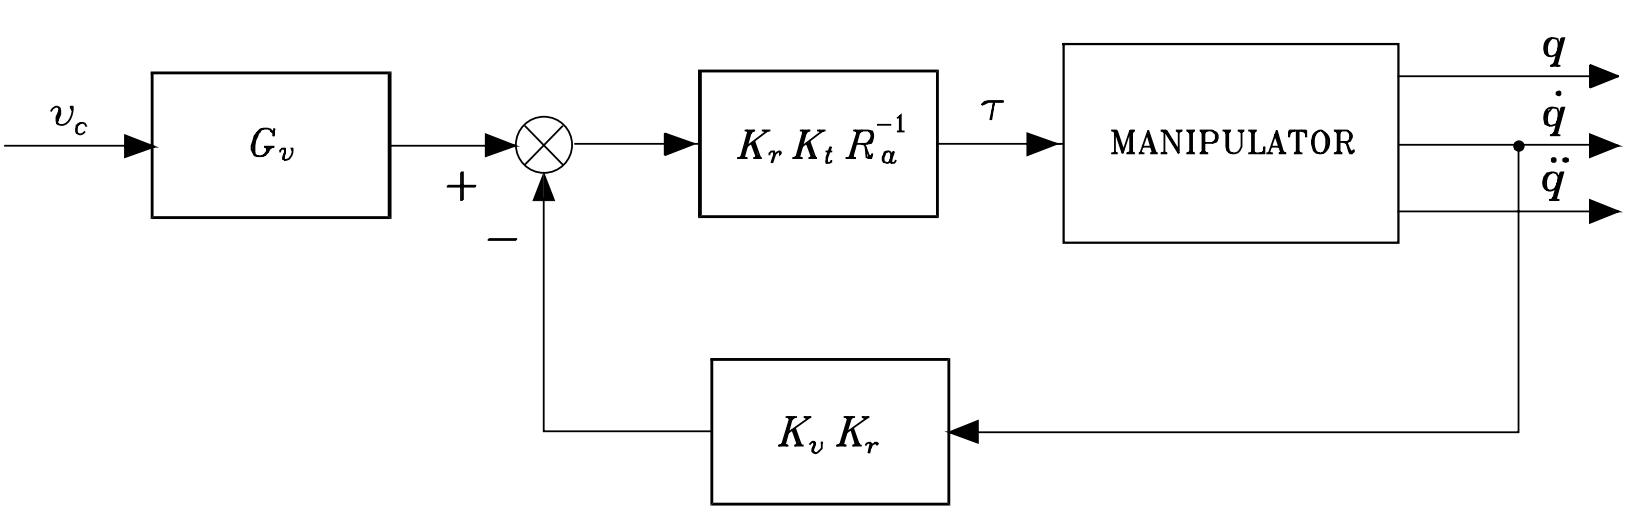
\includegraphics[width=0.75\linewidth]{images/voltage_controlled_1.png}
        \caption{Block scheme of the manipulator and drives system as a voltage-controlled system (source:~\cite{sciavicco2010robotics}).}
        \label{fig:voltage_controlled_1}
    \end{figure}

   
    
\end{frame}


\subsection{Decentralized control}

\begin{frame}
	\frametitle{Outline} % Table of contents slide, comment this block out to remove it
	\tableofcontents[currentsection, currentsubsection] % Throughout your presentation, if you choose to use \section{} and \subsection{} commands, these will automatically be printed on this slide as an overview of your presentation
\end{frame}

\begin{frame}[allowframebreaks]
\frametitle{Decentralized control}

    We can design an independent controller based on the previous scheme only if we assume the following:

    \begin{itemize}
        \item High-ratio gears: the elements of $\mathbf{K}_r$ (transmissions) are much greater than unity. 
        \item High-efficiency servomotors: the elements of $\mathbf{R}_a$ are very small.
        \item The values of $\boldsymbol{\tau}$ required for executing the motions are not too large
    \end{itemize}

    Then, we can assume that
    \begin{equation}
        \mathbf{G}_v\mathbf{v}_c \simeq \mathbf{K}_v\mathbf{K}_r\dot{\mathbf{q}}
        \label{eq:approx_decentralized_control}
    \end{equation}
    
    There is a proportional relatinship between $\mathbf{v}_c$ and $\dot{\mathbf{q}}$ independent to the manipulator parameters. 

    \framebreak
    
    This assumption is more valid the smaller the joint velocities and accelerations.

    Hence, velocity (or voltage) control is more robust w.r.t. the manipulator dynamics parameters, which is enhanced by the values of gear reduction ratios.

    Then, 
    $$
    \mathbf{v}_c \simeq \mathbf{G}_v^{-1}\mathbf{K}_v\mathbf{K}_r\dot{\mathbf{q}}
    $$
    implies that the velocity of the i-th joint $\dot{\mathbf{q}}_i$ depends only on the i-th control voltage ($\mathbf{v}_{c_i}$, since $\mathbf{G}_v^{-1}\mathbf{K}_v\mathbf{K}_r$ is diagonal.

    Therefore, the joint position control system can be designed according to a decentralized control structure: each joint can be controlled independently. 

    \framebreak

    Therefore, under a decentralized control schema:
    \begin{itemize}
        \item The manipulator is conceived as formed by $n$ independent systems and control each joint axis as a SISO system.
    
        \item Interaction and coupling effects between the joints are considered as disturbances acting on each single joint drive system.

        \item The joint controller must guarantee good performance in terms of high disturbance rejection and trajectory tracking capabilities.

        \item Hence, we can apply PID-like controllers to each joint actuator (more on that in~\cite{lynch2017modern}, sections 11.3 and 11.4, in~\cite{sciavicco2010robotics}, section 8.3, and in~\cite{corke_robot_joint_control}). 
    \end{itemize}
    
\end{frame}

\subsection{Centralized control}

\begin{frame}
	\frametitle{Outline} % Table of contents slide, comment this block out to remove it
	\tableofcontents[currentsection, currentsubsection] % Throughout your presentation, if you choose to use \section{} and \subsection{} commands, these will automatically be printed on this slide as an overview of your presentation
\end{frame}

\begin{frame}[allowframebreaks]
\frametitle{Centralized control}
	BUT, if we consider that
    \begin{itemize}
        \item the desired manipulator motion requires large joint speed and/or accelerations,
        \item or if using low-ratio gear reduction or direct-drive actuation ($\mathbf{K}_r = \mathbf{I}$, i.e., the non-linear coupling terms strongly influence the system performance),
    \end{itemize}
    the approximation in equation~\ref{eq:approx_decentralized_control} no longer holds.
    
    Therefore, considering the coupling effects between joints as disturbances may generate large tracking errors. I.e., the decentralized control strategy is not suitable anymore.

    In this case, we can use an inverse dynamics technique to find $\boldsymbol{\tau}(t)$ to track any specified motion in terms of $\ddot{\mathbf{q}}, \dot{\mathbf{q}}, \mathbf{q}$. 

    \framebreak
    This solution is called centralized control and requires the accurate knowledge of the manipulator dynamic model.

   However, we still require the use of error contributions between the desired and the actual trajectory: even if the dynamic model is complex and accurate, it is just an idealization of reality and does not include some effects (Coulomb friction, gear backlash, tolerances, non rigid elements, etc).

    We need to design control algorithms to compensate for the non-linear effects of the manipulator dynamics.

    The manipulator is not a set of $n$ decoupled system but a multi-variable system with $n$ inputs (joint torques) and $n$ outputs (joint motions) integrating between them by means of non-linear relations described in equation~\ref{eq:dynamic_model}.
    
    Non-linear control: see~\cite{sciavicco2010robotics}, Appendix C., for the basics on control of non-linear mechanical systems.
    
\end{frame}

\subsection{Gravity compensation}

\begin{frame}
	\frametitle{Outline} % Table of contents slide, comment this block out to remove it
	\tableofcontents[currentsection, currentsubsection] % Throughout your presentation, if you choose to use \section{} and \subsection{} commands, these will automatically be printed on this slide as an overview of your presentation
\end{frame}

\begin{frame}[allowframebreaks]
\frametitle{Gravity compensation}

One centralized control solution consists of finding the $\boldsymbol{\tau}$ to compensate the dynamics effect of the manipulator. 

Recalling the dynamics that we implemented and tested in \href{https://jmgandarias.com/advanced_robotics/lab2/}{Lab2}, one of the undesired effect is given by the gravity term: it makes the manipulator to "fall". 

Then, we can design a centralized controller that generates the motor torques to compensate these effects by setting the torques of the actuators to be equal to those produced by gravity:
\begin{equation}
    \boldsymbol{\tau} = \mathbf{g}(\mathbf{q})
\end{equation}

\framebreak

Once the gravity terms are compensated, we can add a closed-loop feedback PD controller~\footnote{The mathematical demonstration of why this is a valid controller applying the \textit{Lyapunov direct method} (see~\cite{sciavicco2010robotics}, Appendix C.3.) is given in~\cite{sciavicco2010robotics}, section 8.5.1.} to track the desired joint trajectories.

\begin{figure}
    \centering
    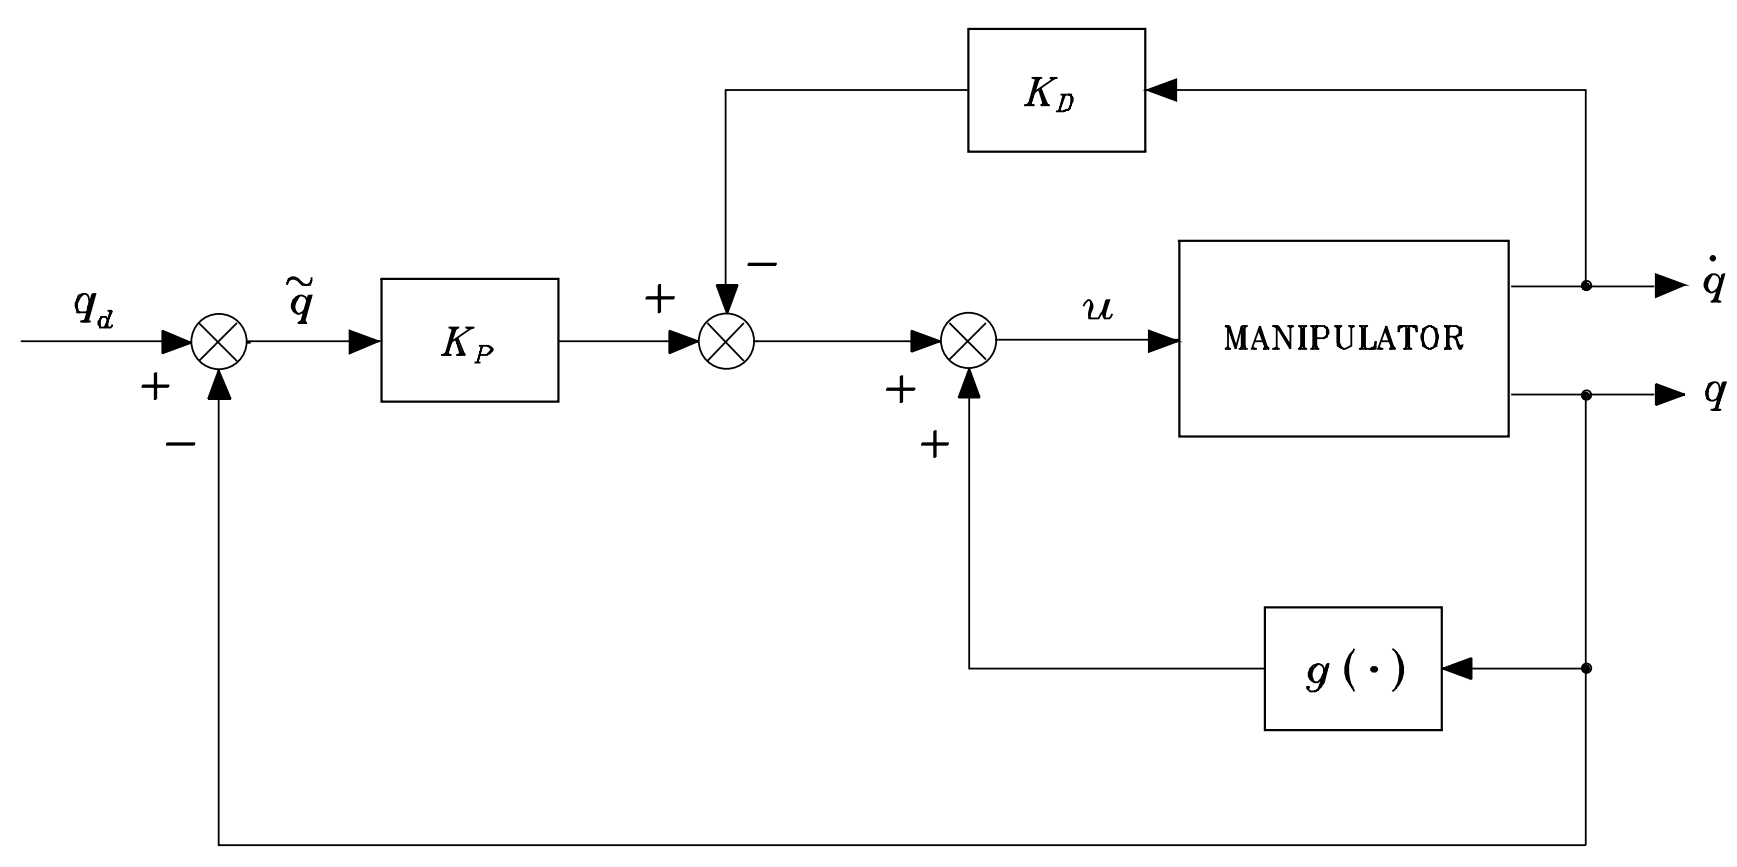
\includegraphics[width=0.6\linewidth]{images/PD_gravity_compensation.png}
    \caption{Joint space PD control with gravity compensation (source~\cite{sciavicco2010robotics}).}
    \label{fig:PD_gravity_compensation}
\end{figure}
	
\end{frame}

\subsection{Inverse dynamics control}


\begin{frame}
	\frametitle{Outline} % Table of contents slide, comment this block out to remove it
	\tableofcontents[currentsection, currentsubsection] % Throughout your presentation, if you choose to use \section{} and \subsection{} commands, these will automatically be printed on this slide as an overview of your presentation
\end{frame}

\begin{frame}[allowframebreaks]
\frametitle{Inverse dynamics control}
	Similarly, we can develop a controller that compensate the whole non-linear manipulator dynamics using an inverse dynamics control approach. 

    The dynamics of an n-joint manipulator in equation~\ref{eq:dynamic_model} can be rewritten as
    \begin{equation}
        \mathbf{M}(\mathbf{q}) \ddot{\mathbf{q}} + \mathbf{n}(\mathbf{q}, \dot{\mathbf{q}}) = \boldsymbol{\tau}
        \label{eq:inverse_dynamics_control}
    \end{equation}
    where
    $$ \mathbf{n}(\mathbf{q}, \dot{\mathbf{q}}) = \mathbf{C} (\mathbf{q}, \dot{\mathbf{q}}) \dot{\mathbf{q}} + \mathbf{F}_b \dot{\mathbf{q}} + \mathbf{g}
    $$

    It is desired to perform not an approximate linearization but an exact linearization of system dynamics obtained by means of a non-linear state feedback. This technique uses a method called \textit{feedback linearization}, a common strategy employed in nonlinear control.

    \framebreak
    
    This is only possible due to the particular form of~\ref{eq:dynamic_model}. In fact, taking the control variable $\mathbb{u}$ as a function of the manipulator state in the form
    $$
    \boldsymbol{u} = \mathbf{M}(\mathbf{q}) y + \mathbf{n}(\mathbf{q}, \dot{\mathbf{q}})
    $$
    leads to the system described by
    $$
    \ddot{\mathbf{q}} = \mathbf{y},
    $$
    where $\mathbf{y}$ represents an input vector determined by the desired dynamic behavior of the manipulator. 

    Hence, using the following nonlinear control law (a.k.a. inverse dynamics control, since it is based on the computation of manipulator inverse dynamics) 
    $$
    \boldsymbol{\tau} = \mathbf{M}(\mathbf{q}) \ddot{\mathbf{q}}_d   + \mathbf{n}(\mathbf{q}, \dot{\mathbf{q}})
    $$
    is linear and decoupled w.r.t. the new input $\ddot{\mathbf{q}}_d$. I.e., the i-th component $\ddot{\mathbf{q}}_{d_i}$ influences with a double integrator relationship, only the variable $\mathbf{q}_i$ independenlty of the motions of the other joints.

    \framebreak

    \begin{figure}
        \centering
        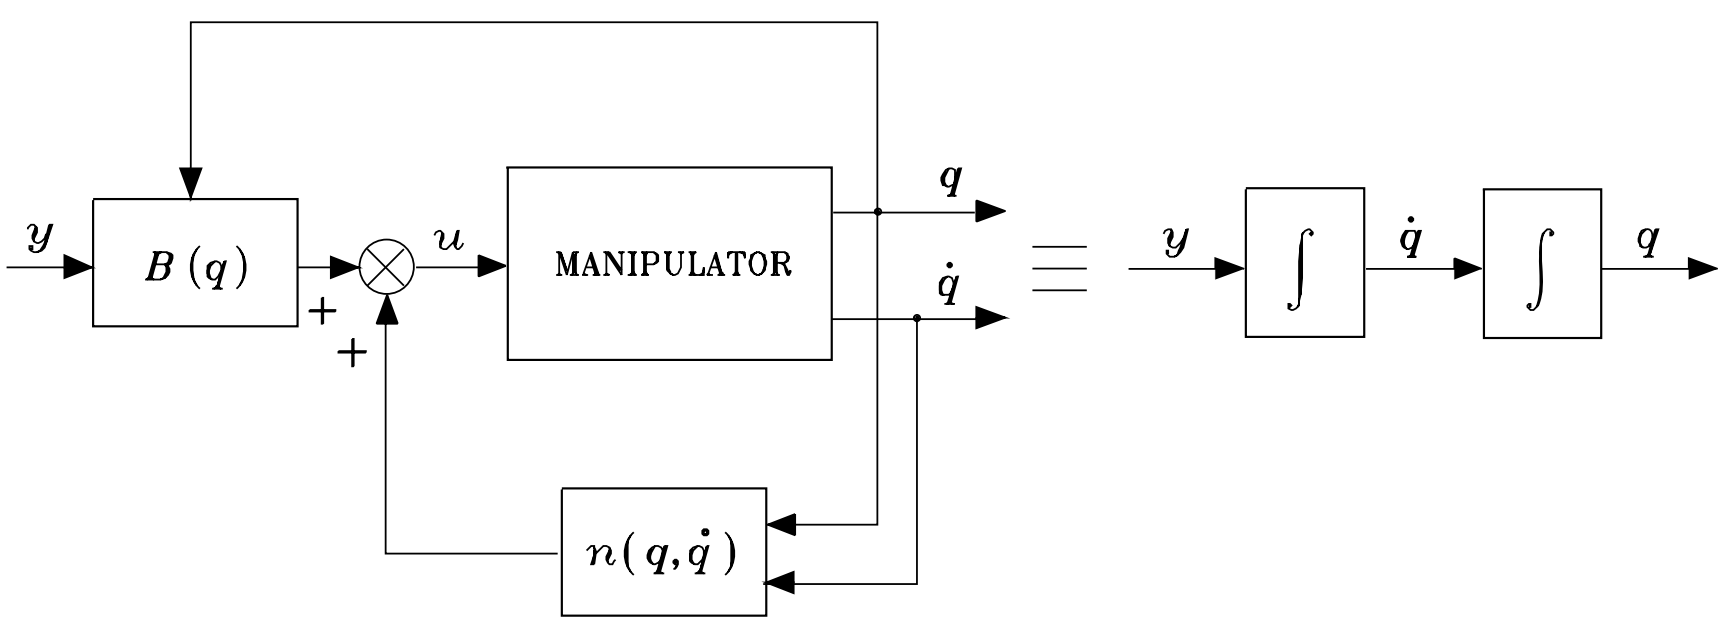
\includegraphics[width=0.75\linewidth]{images/exact_linearization.png}
        \caption{Exact linearization performed by inverse dynamics control (source:~\cite{sciavicco2010robotics}).}
        \label{fig:exact_linearization}
    \end{figure}

    A double integrator system is critically unstable, meaning any input or perturbation will make the system unstable. 

    \framebreak

    Hence, once the non-linear dynamics are compensated, the manipulator control problem is to find a stabilizing control law. For example, a PD controller:

    \begin{figure}
        \centering
        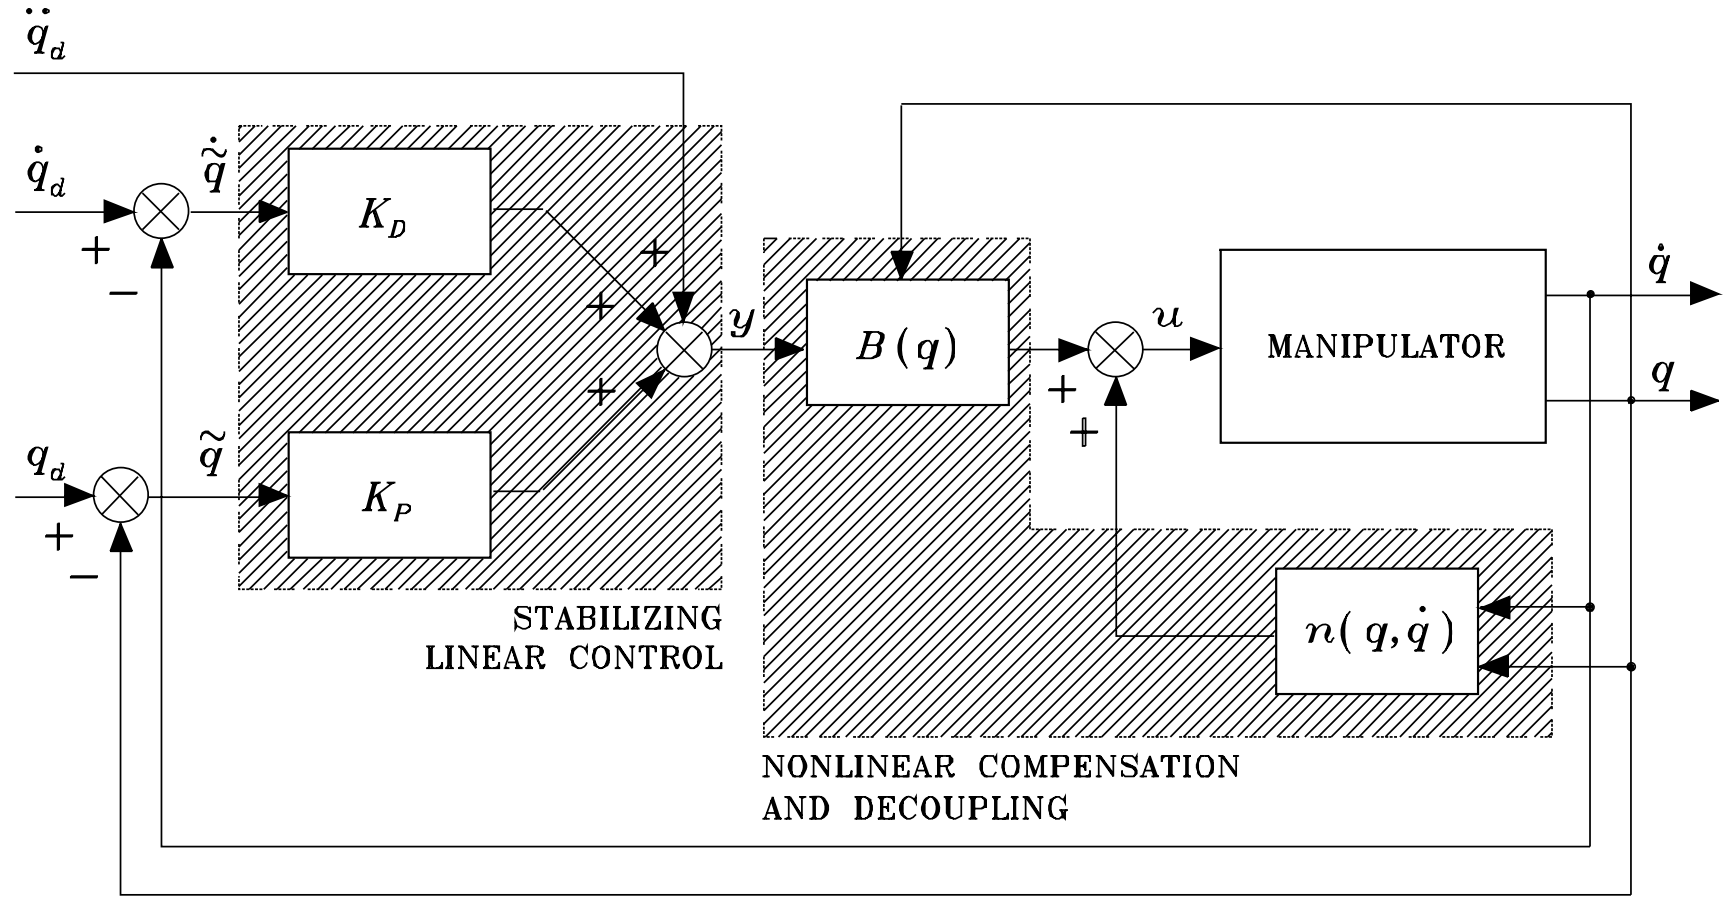
\includegraphics[width=0.7\linewidth]{images/joint_space_inverse_dynamics_control.png}
        \caption{Block scheme of joint space inverse dynamics control (source:~\cite{sciavicco2010robotics}).}
        \label{fig:joint_space_inverse_dynamics_control}
    \end{figure}

    \framebreak
    
    By doing this, the whole system dynamics is defined by the homogeneous second-order differential equation
    $$
    \ddot{\tilde{\mathbf{q}}} +  \mathbf{K}_D \dot{\tilde{\mathbf{q}}}  +  \mathbf{K}_P \ddot{\tilde{\mathbf{q}}}  = \boldsymbol{0}
    $$
    expressing the dynamics of position error while tracking the given trajectory. The error converges to zero depending on the matrices $\mathbf{K}_D$ and $\mathbf{K}_P$. Under the assumption of diagonal and positive definite matrices, the system is asymptotically stable and the dynamic behavior is given by 
    $$
    \mathbf{K}_P = diag\{w_{n_1}^2, \dots, w_{n_n}^2 \} \quad \quad \mathbf{K}_D = diag\{2 \zeta_1 w_{n_1}, \dots, 2 \zeta_n w_{n_n} \}
    $$

    \framebreak

    The implementation of this control scheme requires the online computation of the dynamics model.

    This technique is based on the assumption of perfect cancellation of dynamic terms, which requires that parameters of the dynamic model are accurately known and real-time computation of manipulator dynamics.
    
    This is hard to do in practice due to different sources of uncertainty: imperfect knowledge of manipulator mechanics, unmodelled dynamics, etc.  

    Also, inverse dynamics computation is to be performed at sampling times of a millisecond to ensure that the assumption of operating in the continuous time domain is realistic. 

    Hence, as dynamics compensation may be imperfect, \textit{Robust Control} techniques can be deployed to counteract these effects (see~\cite{sciavicco2010robotics}, section 8.5.3.). 

    
\end{frame}

\section{Operational Space Control}

\begin{frame}
	\frametitle{Outline} % Table of contents slide, comment this block out to remove it
	\tableofcontents[currentsection] % Throughout your presentation, if you choose to use \section{} and \subsection{} commands, these will automatically be printed on this slide as an overview of your presentation
\end{frame}

\begin{frame}[allowframebreaks]
	\frametitle{Operational Space Control} 

    \begin{itemize}
        \item If the motion is specified in terms of operational space variables, the measured joint space variables can be transformed into the corresponding operational space variables through kinematics relations (higher algorithmic complexity).
        \item Advantage: The controller directly acts on the operational space variables. 
        \item However, measuring operational space variables is often performed through evaluation of forward kinematics based on joint space variables measurements.
        \item Basis of control of the interaction with the environment. Joint control schemes suffice only for motion control in the free space. When the manipulator's EE is in contact with the environment it is necessary to control both position and force at the operational space level.
        \item The control schemes are analogous to joint space control schemes, but joint states variables given by the robot sensors are firstly kinematically inverted into the operational space.
    \end{itemize}
    
\end{frame}

\subsection{Gravity compensation}

\begin{frame}
	\frametitle{Outline} % Table of contents slide, comment this block out to remove it
	\tableofcontents[currentsection, currentsubsection] % Throughout your presentation, if you choose to use \section{} and \subsection{} commands, these will automatically be printed on this slide as an overview of your presentation
\end{frame}

\begin{frame}[allowframebreaks]
\frametitle{Gravity compensation}

    \begin{figure}
        \centering
        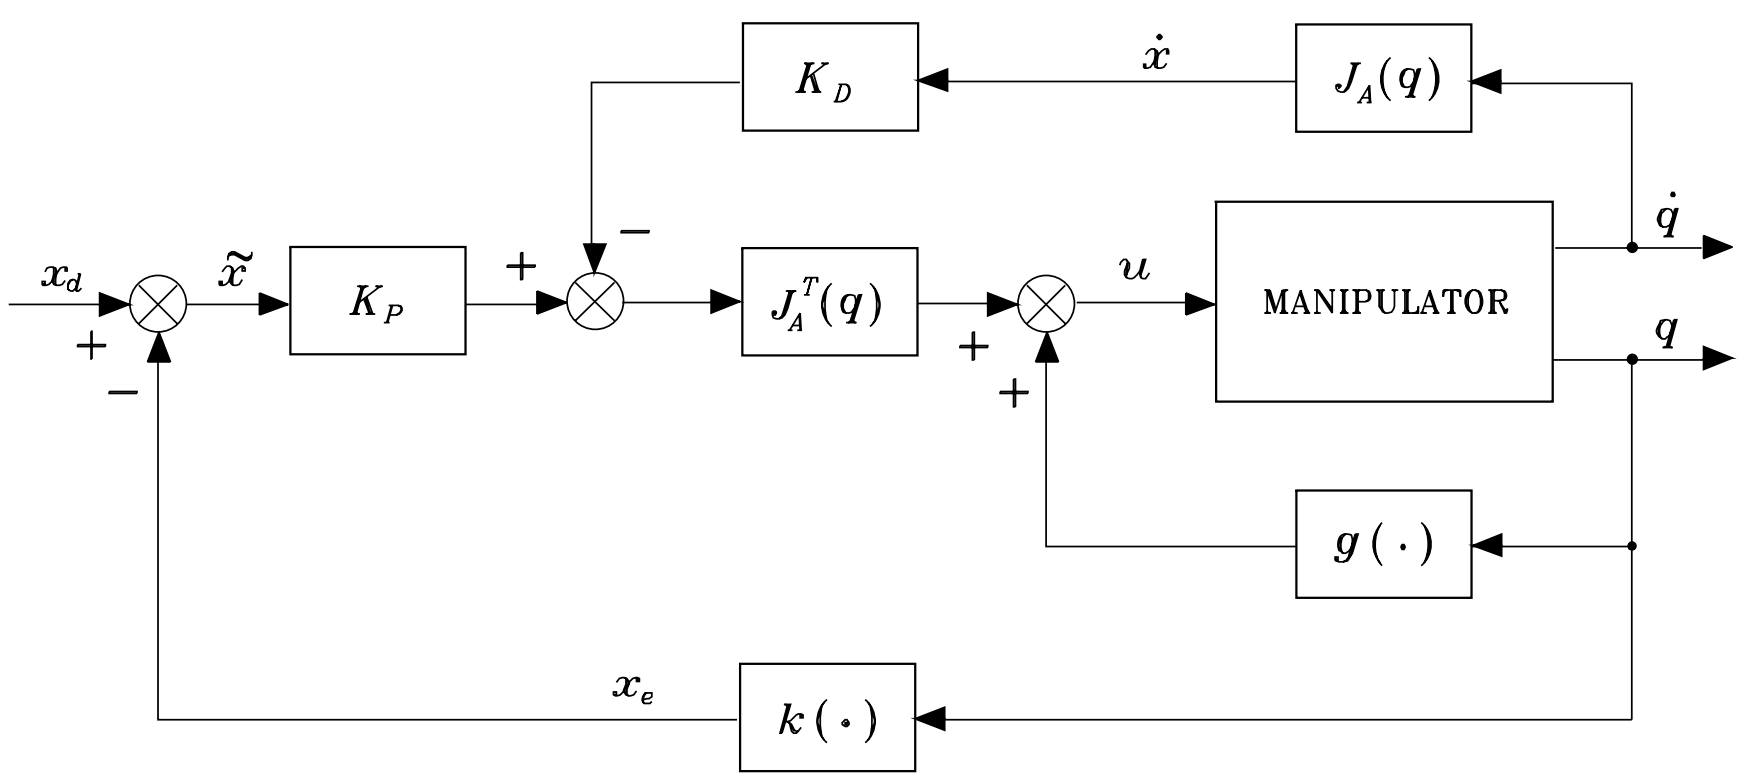
\includegraphics[width=0.75\linewidth]{images/gravity_compensation_operational.png}
        \caption{Block scheme of operational space PD control with gravity compensation (source:~\cite{sciavicco2010robotics}).}
        \label{fig:gravity_compensation_operational}
    \end{figure}
    
\end{frame}

\subsection{Inverse dynamics control}

\begin{frame}
	\frametitle{Outline} % Table of contents slide, comment this block out to remove it
	\tableofcontents[currentsection, currentsubsection] % Throughout your presentation, if you choose to use \section{} and \subsection{} commands, these will automatically be printed on this slide as an overview of your presentation
\end{frame}

\begin{frame}[allowframebreaks]
\frametitle{Inverse dynamics control}

\begin{figure}
    \centering
    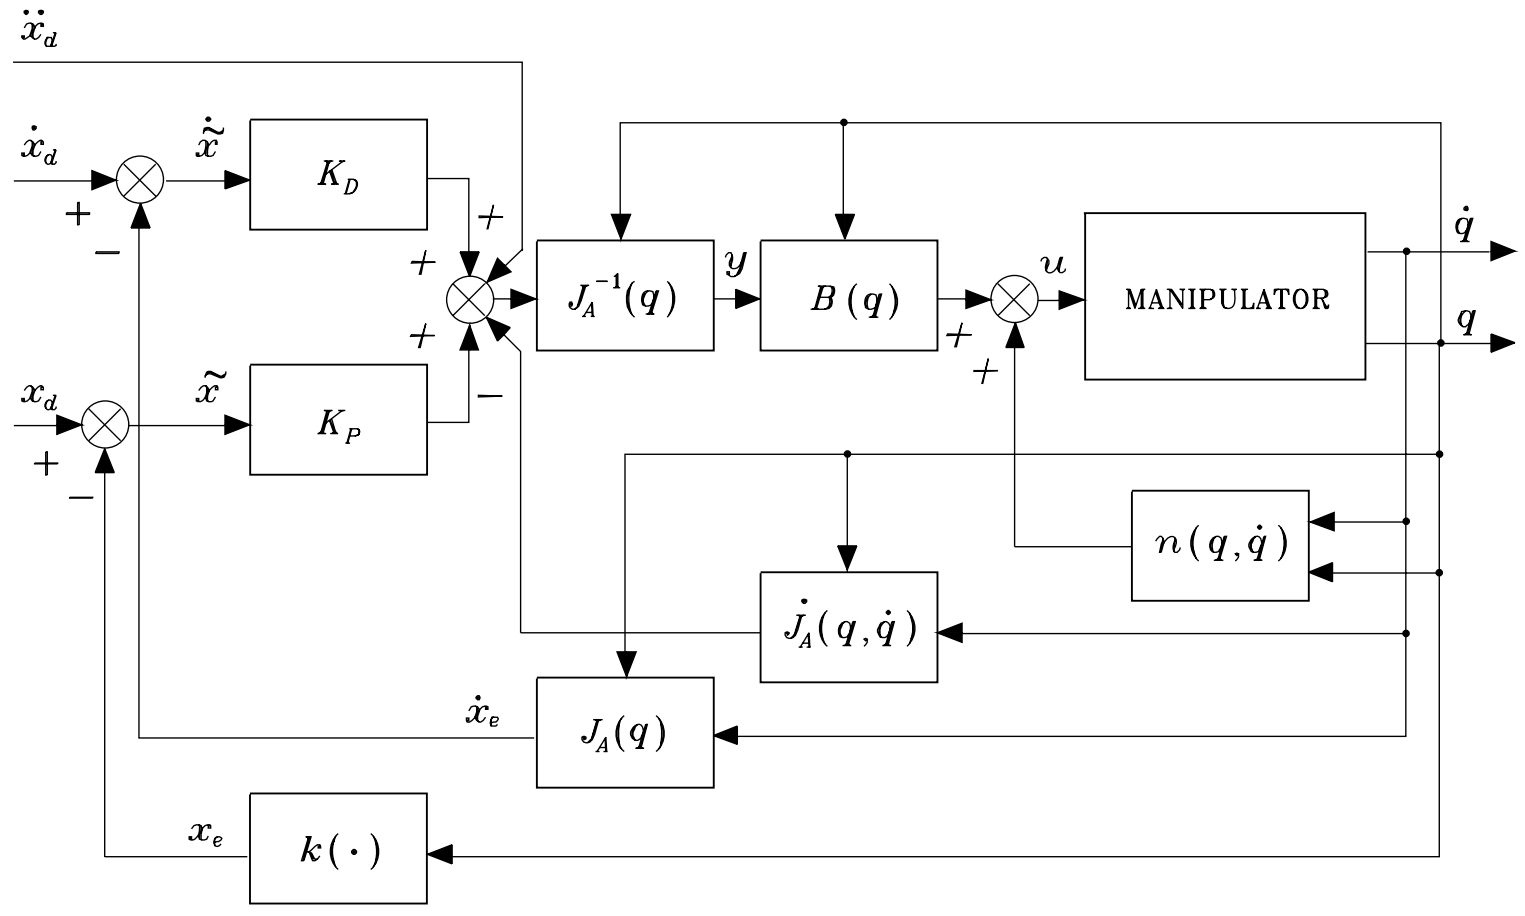
\includegraphics[width=0.7\linewidth]{images/inverse_dynamics_control_operational.png}
    \caption{Block scheme of operational space inverse dynamics control (source:~\cite{sciavicco2010robotics}).}
    \label{fig:inverse_dynamics_control_operational}
\end{figure}
    
\end{frame}



\begin{frame}[allowframebreaks]
\frametitle{Bibliography}
\printbibliography
\end{frame}

\end{document}